\documentclass[slidestop,compress,mathserif]{beamer}
%\documentclass[slidestop,compress,mathserif,handout]{beamer}

%\documentclass[xcolor=dvipsnames,handout]{beamer}
%\documentclass[xcolor=dvipsnames]{beamer}

%\documentclass[handout]{beamer}

%%% To get rid of solutions on handouts:
\newcommand{\soln}[1]{\textit{\textcolor{darkGray}{#1}}}				% For slides
%\newcommand{\soln}[1]{ }	% For handouts

% to get pausing to work properly on slides
\newcommand{\hide}[1]{#1}	% For slides
%\newcommand{\hide}[1]{ }	% For handouts


\input{../LectureStyle.tex}

%%%%%%%%%%%%%%%%%%%%%%%%%%%%%%%%%%%%%%%%%%%%%%%%%%%%%%%%%%%%%%%%%%%%%%%%%%%%%%%%%%%%%%%%%%%%%%%
\title[Chapter 5 part 2]{Chapter 5 part 2}
\subtitle{Continuous Random Variables}

%%%%%%%%%%%%%%%%%%%%%%%%%%%%%%%%%%%%%%%%%%%%%%%%%%%%%%%%%%%%%%%%%%%%%%%%%%%%%%%%%%%%%%%%%%%%%%%


\author[Jingchen (Monika) Hu] % (optional, use only with lots of authors)
{Jingchen (Monika) Hu}
% - Give the names in the same order as the appear in the paper.
% - Use the \inst{?} command only if the authors have different
%   affiliation.

\institute[Vassar] % (optional, but mostly needed)
{Vassar College}
% - Use the \inst command only if there are several affiliations.
% - Keep it simple, no one is interested in your street address.

\date[MATH 241] % (optional, should be abbreviation of conference name)
{MATH 241}
% - Either use conference name or its abbreviation.
% - Not really informative to the audience, more for people (including
%   yourself) who are reading the slides online

\subject{MATH 241}
% This is only inserted into the PDF information catalog. Can be left
% out.



% If you wish to uncover everything in a step-wise fashion, uncomment
% the following command:

%\beamerdefaultoverlayspecification{<+->}



\begin{document}




%%%%%%%%%%%%%%%%%%%%%

% Title Page

\begin{frame}%[plain]
\titlepage
\end{frame}


%%%%%%%%%%%%%%%%%%%%%%%%%%%%%%%%%%%%%%%%%%
%\addtocounter{framenumber}{-1}
%\begin{frame}{Midterm Feedback}
%\begin{columns}[T]
%\begin{column}{4cm}
%\vspace{-1cm}
%\begin{figure}
%\centering
%\includegraphics[width=5cm,height=8cm]{figures/feedback_barplots}
%\end{figure}
%\end{column}
%\begin{column}{7.8cm}
%\vspace{-0.3cm}
%{\pause
%\small \centerline{\underline{\textbf{Likes}}}}
%{%\footnotesize
%\begin{itemize}
%\item Lecture: well-organized, informative, \\
%clear expectation, good balance between theory and practice
%%in-class questions are  %\\``one of the best math classes"
%\item Slides: well-prepared, easy to follow
%%\item In-class questions: very helpful
%\item Homework \& quizzes: good practice
%\item In-class questions: helpful %in understanding concepts
%\item Exam \& quizzes: fair in difficulty
%\item ``Somewhat challenging but not too much''
%%\item Willingness to help%Available outside of classroom %office hour
%%\item Lab: interesting, practical programming skill, solidify core concepts
%\end{itemize}
%}
%{\pause
%\small \centerline{\underline{\textbf{To improve}}}}
%{%\footnotesize
%\begin{itemize}
%%\item Detailed expectation on the programming software (R) in syllabus
%\item Examples in class: more similar to HW %(harder)
%\item Homework solutions
%\item Practice exam
%%\item Post slides 12 hours before class
%%\item Go over commonly missed homework in class
%%\item Increase participation for in-class questions
%%\item More in-class activities (?)
%%\item More explanation in labs
%%\item More video?
%%\item Slides on Sakai: same slides or handout?
%%\item More practice, more examples
%%\item Some other detailed suggestions...
%
%\end{itemize}
%}
%\end{column}
%\end{columns}
%\end{frame}


%%%%%%%%%%%%%%%%%%%%%%
%\addtocounter{framenumber}{-1}
%
%\begin{frame}\frametitle{Annoucement}
%
%\begin{itemize}
%%\item HW5: \red{due now!}
%\item HW6: \red{due Thursday, Oct 23nd}
%
%\vspace{0.5cm}
%
%
%
%\end{itemize}
%%\begin{center}
%%\includegraphics[width = \textwidth]{figures/midterm_score}
%%\end{center}
%
%
%\end{frame}



%%%%%%%%%%%%%%%%%%%%%%
\begin{frame}{Outline}
%\tableofcontents[hideallsubsections,pausections]
\tableofcontents[hideallsubsections]
\end{frame}
%%%%%%%%%%%%%%%%%%%%%%%%%%%%%%%%%%%%%%%%%%
\section{Normal distribution}
%%%%%%%%%%%%%%%%%%%%%%%%%%%%%%%%%%%%%%%%%%

\begin{frame}
\frametitle{Normal Distribution}

\vspace{-0.2cm}
\begin{defn}
A continuous random variable $X$ has a \hl{Normal distribution} distribution with mean $\mu$ and variance $\sigma^2$ if its pdf is
%\vspace{-0.3cm}
\[
X \sim \text{N}(\mu, \sigma^2) \Longleftrightarrow
 f(x) = \frac{1}{\sqrt{2\pi\sigma^2}}~e^{ -\frac{(x-\mu)^2}{2\sigma^2} }, \text{ where } x \in \mathbb{R}
\]
\end{defn}

Pdf: unimodal and symmetric, bell shaped random variable
\begin{center}
\includegraphics[width = 0.5\textwidth]{figures/normal_pdf}
\end{center}

\end{frame}


%%%%%%%%%%%%%%%%%%%%%%%%%%%%%%%%%%%%%
%\addtocounter{framenumber}{-1}
%\begin{frame}
%\frametitle{Get yourself a 10 Deutsche Mark bill}
%
%\begin{center}
%\includegraphics[width=\textwidth]{figures/deutsche_mark}
%\end{center}
%
%\end{frame}


%%%%%%%%%%%%%%%%%%%%%%%%%%%%%%%%%%%%%%%%%%
\begin{frame}\frametitle{The normal pdf is well-defined} %$f(x)= \frac{1}{\sqrt{2\pi\sigma^2}}~e^{ -\frac{1}{2}\frac{(x-\mu)^2}{\sigma^2} }$}
({\color{red}not required})
\[\int_{-\infty}^\infty \frac{1}{\sqrt{2\pi\sigma^2}}~e^{ -\frac{(x-\mu)^2}{2\sigma^2} } dx =1 \]
\cl{Use the fact that normal pdf is well define, calculate the integral
\[
\int_{-\infty}^{\infty} e^{-\frac{(x + 2)^2}{6}}dx = ?
\]
}
\pause
Suppose we have a random variable $X \sim \text{N}(\mu = -2, \sigma^2 = 3)$, then
\[
1  = \int_{-\infty}^\infty \frac{1}{\sqrt{2\pi\sigma^2}}~e^{ -\frac{(x-\mu)^2}{2\sigma^2} } dx
 = \int_{-\infty}^{\infty} \frac{1}{\sqrt{2 \pi \cdot 3}}~e^{-\frac{(x +2 )^2}{6}}dx\]
 \[\Longrightarrow \int_{-\infty}^{\infty} e^{-\frac{(x + 2)^2}{6}}dx = \sqrt{6\pi}\]




\end{frame}


%%%%%%%%%%%%%%%%%%%%%%%%%%%%%%%%%%%%

\begin{frame}
\frametitle{Normal distributions with different parameters}

\vspace{-1cm}
\begin{center}
\[N(\mu = 0, \sigma^2 = 1) \hspace{1.4cm} N(\mu = 19, \sigma^2 = 16) \]
\includegraphics[width=0.7\textwidth]{figures/twoSampleNormals}
\end{center}

\begin{center}
\includegraphics[width=0.7\textwidth]{figures/twoSampleNormalsStacked}
\end{center}

\end{frame}

%%%%%%%%%%%%%%%%%%%%%%%%%%%%%%%%%%%%%%%%%%
\begin{frame}\frametitle{Mean and variance of Normal random variable}
If $X \sim \text{N}(\mu, \sigma^2)$, and $Z = \frac{X - \mu}{\sigma}$, then $Z$ has a standard normal distribution (more later in Chapter 5.7).
%\vspace{-0.2cm}
\[ Z \sim \text{N}(0, 1) \]
%\red{Proof}


\begin{itemize}
\item $E[X] = \mu$ ({\color{red} required})
\end{itemize}



%\red{Proof}
%\invisible{
%\pause
\hspace{0.5cm}
Since $X \sim \text{N}(\mu, \sigma^2) \Longleftrightarrow X = \sigma Z + \mu$ and $Z \sim \text{N}(0, 1)$,
it's suffice to show the mean and variance of standard normal are $0$ and $1$.

{\footnotesize{
\begin{align*}
E[Z] & = \int_{-\infty}^{\infty} x f_Z(x) dx = \int_{-\infty}^{\infty} x \frac{1}{\sqrt{2\pi}} e^{-\frac{x^2}{2}}dx\\
& = \frac{1}{\sqrt{2\pi}}\int_{-\infty}^{\infty} x~e^{-\frac{x^2}{2}}dx\\
& = -\frac{1}{\sqrt{2\pi}}\left. e^{-\frac{x^2}{2}}\right|_{-\infty}^{\infty} = 0
\end{align*}
}}
%}

\end{frame}

%%%%%%%%%%%%%%%%%%%%%%%%%%%%%%%%%%%%%%%%%%
\begin{frame}\frametitle{Mean and variance of Normal random variable}
If $X \sim \text{N}(\mu, \sigma^2)$, and $Z = \frac{X - \mu}{\sigma}$, then $Z$ has a standard normal distribution (more later in Chapter 5.7).
%\vspace{-0.2cm}
\[ Z \sim \text{N}(0, 1) \]
%\red{Proof}

\begin{itemize}
\item $Var(X) = \sigma^2$ ({\color{red} required})
\end{itemize}


%\red{Proof}
%\invisible{
%\pause
\hspace{0.5cm}
Since $X \sim \text{N}(\mu, \sigma^2) \Longleftrightarrow X = \sigma Z + \mu$ and $Z \sim \text{N}(0, 1)$,
it's suffice to show the mean and variance of standard normal are $0$ and $1$.

{\footnotesize{
\begin{align*}
Var[Z] & = E[Z^2]  - (E[Z])^2 = E[Z^2] = \int_{-\infty}^{\infty} x^2 f_Z(x) dx = \int_{-\infty}^{\infty} x^2 \frac{1}{\sqrt{2\pi}} e^{-\frac{x^2}{2}}dx\\
& = \frac{1}{\sqrt{2\pi}}\int_{-\infty}^{\infty} x^2~e^{-\frac{x^2}{2}}dx \,\,\, (\text{integration by parts}: u = x, dv = xe^{-x^2/2}dx) \\
& = \frac{1}{\sqrt{2\pi}}\left\{  - \left. xe^{-\frac{x^2}{2}}\right|_{-\infty}^{\infty} + \int_{-\infty}^{\infty} e^{-\frac{x^2}{2}}dx\right\}\\
& = \int_{-\infty}^{\infty} \frac{1}{\sqrt{2\pi}}e^{-\frac{x^2}{2}}dx =1
\end{align*}
}}

\end{frame}


%%%%%%%%%%%%%%%%%%%%%%%%%%%%%%%%%%%%

\begin{frame}
\frametitle{68-95-99.7 Rule}

\begin{itemize}

\item A random variable $X$ has a normal distribution,
\begin{itemize}
\item about 68\% probability $X$ falls within 1 SD of the mean,
\item about 95\% probability $X$ falls within 2 SD of the mean,
\item about 99.7\% probability $X$ falls within 3 SD of the mean.
\end{itemize}

\item The probability of $X$ falls 4, 5, or more standard deviations away from the mean is very low.

\end{itemize}

\begin{center}
\includegraphics[width=0.7\textwidth]{figures/6895997}
\end{center}

\end{frame}




%%%%%%%%%%%%%%%%%%%%%%%%%%%%%%%%%%%%%%%%%%
\begin{frame}\frametitle{Normal probability calculation}
\begin{itemize}
%\item If $X \sim \text{N}(\mu, \sigma^2)$, and $Z = \frac{X - \mu}{\sigma}$, then $Z$ has a standard normal distribution.
%%\vspace{-0.2cm}
%\[ Z \sim \text{N}(0, 1) \]
%%\red{Proof}
%\pause
%We are going to show this later, when we learn Chapter 5.7.

%%\invisible{
%\pause\vspace{-0.5cm}%\footnotesize{
%\[ X  = \sigma Z + \mu  \Longrightarrow \]
%\[ F_Z(z)   = P(Z \leq z) = P(X \leq \sigma z + \mu) = F_X(\sigma z + \mu) \]
%\pause\vspace{-0.5cm}
%\begin{align*}
%f_Z(z) &  = \frac{d}{dz}F_Z(z) =  \frac{d}{dz} F_X(\sigma z + \mu)\\
%\text{\red{(chain rule)}}  &  =  f_X(\sigma z + \mu) \cdot \frac{d}{dz} (\sigma z + \mu)\\
%& =  \frac{1}{\sqrt{2\pi\sigma^2}}~e^{ -\frac{1}{2}\frac{(\sigma z + \mu-\mu)^2}{\sigma^2} } \cdot \sigma
% =  \frac{1}{\sqrt{2\pi}}~e^{ -\frac{1}{2}z^2 }
%\end{align*}
%%}
%%}

%\pause
\item We denote $\phi(x)$ and $\Phi(x)$ as pdf and cdf of the standard normal distribution respectively.

\item Probability calculations for $X$ in terms of $Z$:
\begin{align*}
P(a < X < b) %&= P\left(\frac{a - \mu}{\sigma} < \frac{X - \mu}{\sigma} \leq \frac{b - \mu}{\sigma}\right)\\
&= P\left(\frac{a - \mu}{\sigma} < Z < \frac{b - \mu}{\sigma}\right) \\
%&= P\left(Z \leq \frac{b - \mu}{\sigma} \right) - P\left(Z \leq \frac{a - \mu}{\sigma}\right) \\
& = \Phi\left(\frac{b - \mu}{\sigma}\right) - \Phi\left(\frac{a - \mu}{\sigma}\right)
\end{align*}


\end{itemize}
\end{frame}


%%%%%%%%%%%%%%%%%%%%%%%%%%%%%%%%%%%%

\begin{frame}
\frametitle{}

\twocol{0.45}{0.55}
{
\begin{center}
\includegraphics[width=\textwidth]{figures/keep_calm2}
\end{center}
}
{

\cl{Using the 68-95-99.7 rule, find the standard normal cdf $\Phi(-2)$ and $\Phi(2)$}

%\invisible{
\pause
\begin{align*}
\Phi(-2) = & P(Z < -2) \\
& = \frac{1- P(-2 < Z < 2)}{2} \\
& = \frac{1-0.95}{2} = 0.025
\end{align*}

\pause
\[ \Phi(2) = 1 - \Phi(-2) = 0.975 \]

%}

}
\end{frame}

%%%%%%%%%%%%%%%%%%%%%%%%%%%%%%%%%%%%
\begin{frame}

\cl{{At Heinz ketchup factory the amounts which go into bottles of ketchup are supposed to be normally distributed with mean 36 oz. and standard deviation 0.11 oz. Once every 30 minutes a bottle is selected from the production line, and its contents are noted precisely. If the amount of ketchup in the bottle is below 35.8 oz. or above 36.2 oz., then the bottle will fails the quality control inspection. What percent of bottles \underline{pass} the quality control inspection?}}


\pause
\[ X \sim \text{N}(36, 0.11^2), \quad P(35.8 < X < 36.2) = ? \]

\end{frame}

\begin{frame}
\[ X \sim \text{N}(36, 0.11^2), \quad P(35.8 < X < 36.2) = ? \]

\begin{columns}[c]
\column{0.3\textwidth}

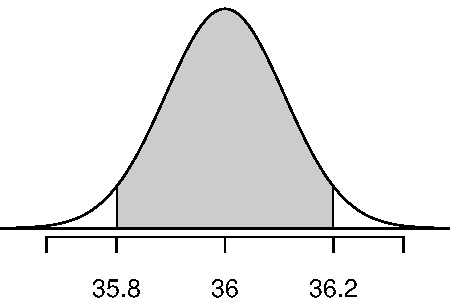
\includegraphics[width=\textwidth]{figures/ketchupBET}
\column{0.05\textwidth}
=
\column{0.3\textwidth}
\includegraphics[width=\textwidth]{figures/ketchupLT362}
\column{0.05\textwidth}
-
\column{0.3\textwidth}
\includegraphics[width=\textwidth]{figures/ketchupLT358}
\end{columns}
\pause
\[z_1 = \frac{35.8 - 36}{0.11} = -1.82, \quad
z_2 = \frac{36.2 - 36}{0.11} = 1.82
\]
\begin{align*}
P(35.8 < X < 36.2) &= P(-1.82 < Z < 1.82) \\
&= P(Z < 1.82) - P(Z < -1.82) \\
&= 0.9656 - 0.0344 = 0.9312
\end{align*}

\end{frame}



%%%%%%%%%%%%%%%%%%%%%%%%%%%%%%%%%%%%%%%%%%%
\begin{frame}
\frametitle{Normal approximation to the Binomial distribution}

\vspace{-0.5cm}
\begin{center}
\includegraphics[scale = 0.6]{figures/pmf2}
\end{center}

\end{frame}
%%%%%%%%%%%%%%%%%%%%%%%%%%%%%%%%%%%%%%%%%%



\begin{frame}
\frametitle{Normal approximation to the Binomial distribution}

Let $X \sim \text{Bin}(n, p)$.
When $n$ is large enough, or more specifically, $np (1-p) \geq 10$,
the binomial distribution can be approximated by the normal distribution
\[ P(X = i) \approx P(i - 0.5 < Y < i + 0.5), \quad Y \sim \text{N}(\mu, \sigma^2) \]
with parameters $\mu = np$ and $\sigma^2 = np(1-p)$.

\begin{itemize}
\item Probability calculation (actually, approximation)
\begin{align*}
P(a \leq X \leq b) &\approx P(a - 0.5 < Y < b + 0.5) \\
& = P\left( \frac{a - 0.5 - np}{\sqrt{np(1-p)}} < \frac{Y - \mu}{\sigma} < \frac{b + 0.5 - np}{\sqrt{np(1-p)}} \right)\\
& = \Phi\left( \frac{b + 0.5 - np}{\sqrt{np(1-p)}} \right) -  \Phi\left( \frac{a - 0.5 - np}{\sqrt{np(1-p)}} \right)
\end{align*}



\end{itemize}

\end{frame}


%%%%%%%%%%%%%%%%%%%%%%%%%%%%%%%%%%%%

\begin{frame}
\frametitle{}

\cl{\small A recent study found that ``Facebook users get more than they give". For example:
\vspace{-0.5cm}
\begin{itemize}
\item Users in our sample pressed the like button next to friends' content an average of 14 times, but had their content ``liked" an average of 20 times
\item 12\% of users tagged a friend in a photo, but 35\% were themselves tagged in a photo
\end{itemize}
\vspace{-0.2cm}
This is because there are 	``power users'' who contribute much more content than the typical user.
The same study found that approximately 25\% of Facebook users are considered power users.
It also found that the average Facebook user has 245 friends.
What is the probability that the average Facebook user with 245 friends has 70 or more friends who would be considered power users?}
\pause

\begin{itemize}
\item We are given that $X \sim \text{Bin}(n = 245, p = 0.25)$, and we are asked for the probability
\[
P(X \ge 70) = p(70) + p(71) + \cdots + p(245) = 1 - p(0) - p(1) - \cdots - p(69)
\]

\item \pause To use normal approximation, first check conditions
\[ np(1-p) = 245 \times 0.25 \times 0.75 = 45.94 \geq 10\]
\end{itemize}
\ct{\webURL{http://www.pewinternet.org/Reports/2012/Facebook-users/Summary.aspx}}

\end{frame}

%%%%%%%%%%%%%%%%%%%%%%%%%%%%%%%%%%%%

\begin{frame}
\frametitle{}

\cl{What is the probability that the average Facebook user with 245 friends has 70 or more friends who would be considered power users?}
Use Normal approximation.
\[ \mu = 245 \times 0.25 = 61.25, \quad \sigma = \sqrt{245 \times 0.25 \times 0.75} = 6.78 \]
\[ Y \sim \text{N}(\mu, \sigma^2), \quad P(X \ge 70) \approx P(Y > 70 - 0.5) \]
\pause
\twocol{0.45}{0.55}{
\begin{center}
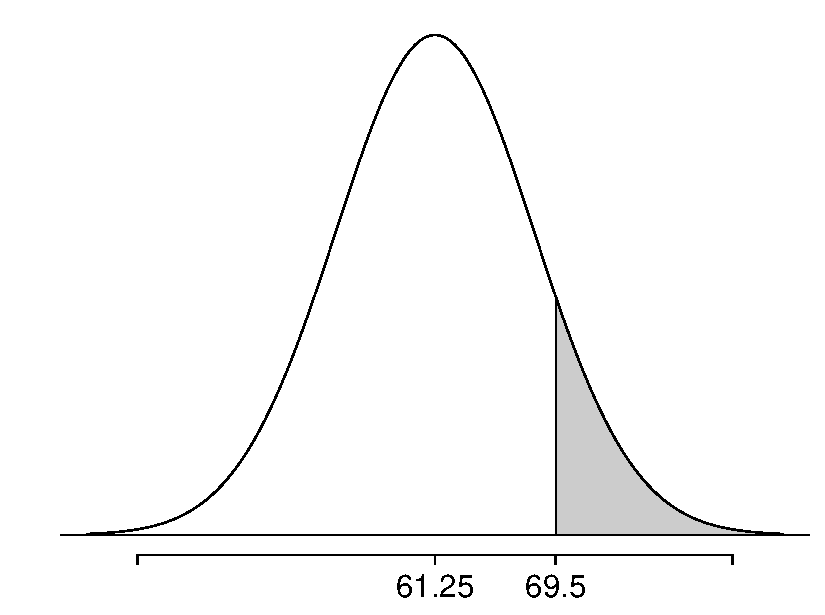
\includegraphics[width=\textwidth]{figures/fbpoweruser_norm}
\end{center}
}
{\pause
\begin{align*}
P(X \ge 70) & \approx P(Y > 70 - 0.5)\\
& = P\left(Z > \frac{\red{69.5} - 61.25}{6.78}\right)\\
& = P(Z > 1.22) \\
&= 1 - 0.8888 = 0.1112
\end{align*}
}


\end{frame}



%%%%%%%%%%%%%%%%%%%%%%%%%%%%%%%%%%%%%%%%%%
\begin{frame}\frametitle{Recap: Normal distribution $X \sim \text{N}(\mu, \sigma^2)$}

\twocol{0.25}{0.75}
{
\begin{center}
\includegraphics[scale = 0.3]{figures/cdf_pos}
\end{center}
\begin{center}
\includegraphics[scale = 0.3]{figures/cdf_neg}
\end{center}
}
{
 %(or Gaussian distribution)
\begin{itemize}
%\vspace{0.2cm}
%\item Pdf \vspace{-0.5cm}
%\[f(x) = \frac{1}{\sqrt{2\pi\sigma^2}}~e^{ -\frac{(x-\mu)^2}{2\sigma^2} } \]
\item Mean $\mu$, variance $\sigma^2$
\item Symmetry \vspace{-0.2cm}
\[ f(\mu-x) = f(\mu+x), F(\mu-x) = 1 - F(\mu+x) \]
\item \vspace{-0.2cm}
Standard normal distribution $\mu = 0, \sigma^2 = 1$. \vspace{-0.2cm}
\[ X \sim \text{N}(\mu, \sigma^2) \Longleftrightarrow Z = \frac{X - \mu}{\sigma} \sim \text{N}(0, 1)\]
\item \vspace{-0.2cm}
Find probability using $\Phi(\cdot)$ table \vspace{-0.2cm}
\[ P(a< X < b) = \Phi\left( \frac{b - \mu}{\sigma}\right) - \Phi\left( \frac{a - \mu}{\sigma}\right) \]
\item \vspace{-0.2cm}
Normal approximation to Binomial $X \sim \text{Bin}(n, p)$ \vspace{-0.2cm}
\[ Y \sim \text{N}(\mu = np, \sigma^2 = np(1-p))\] \[P(X = i) \approx P(i - 0.5 < Y < i + 0.5) \]
\end{itemize}
}


\end{frame}


\begin{frame}\frametitle{Review: continuous distributions}

\begin{center}
\begin{tabular}{lllcc}
\hline
			Name 					& Range 			& pdf $f(x)$																& mean 						& variance \\
\hline
Unif$(\alpha, \beta)$		& $[\alpha, \beta]$	& $\frac{1}{\beta - \alpha}$											& $\frac{\alpha + \beta}{2}$	& $\frac{(\beta - \alpha)^2}{12}$\\
&&&&\\
N$(\mu, \sigma^2)$		& $(-\infty, \infty)$	& $\frac{1}{\sqrt{2\pi\sigma^2}}e^{ -\frac{1}{2}\frac{(x-\mu)^2}{\sigma^2}}$	& $\mu$						& $\sigma^2$\\ 
\hline
\end{tabular}
\end{center}

\end{frame}

%%%%%%%%%%%%%%%%%%%%%%

%%%%%%%%%%%%%%%%%%%%%%%%%%%%%%%%%%%%%%%%%%
\section{Distribution of a function of a continuous random variable}
%%%%%%%%%%%%%%%%%%%%%%%%%%%%%%%%%%%%%%%%%%

\begin{frame}
\frametitle{A (important!) theorem on finding pdf of $g(X)$}
Suppose X is a continuous random variable with pdf $f_X(x)$. If a function $g(x)$ is
\begin{enumerate}
\item monotonic (increasing or decreasing), and
\item differentiable (and thus continuous),
\end{enumerate}
then the random variable defined by $Y = g(X)$ has pdf
\[ f_Y ( y ) = f_X( x )  \left|\frac{dx}{dy}\right| \]
Or more rigorously,
\begin{align*}
f_Y ( y ) =
  \begin{cases}
  f_X\left[ g^{-1}(y) \right] \cdot \left|\frac{d}{dy}g^{-1}(y)\right| & \text{ if } y = g(x) \text{ for some } x \\
  0 													 & \text{ if } y \neq g(x) \text{ for all } x \\
  \end{cases}
\end{align*}

\end{frame}


%%%%%%%%%%%%%%%%%%%%%%%%%%%%%%%%%%%%%
\begin{frame}

\cl{Let $X \sim \text{N}(\mu, \sigma^2)$, what distribution does $Y = (X-\mu)/\sigma$ have?}
\vspace{0.3cm}
\pause
In order to use the previous theorem, follow these steps:
\begin{enumerate}
\item Check if $g(x) = (x-\mu)/\sigma$ is monotonic and differentiable \uncover<3->{\checkmark}
\item Compute the inverse function $y = g(x) \Longleftrightarrow x = g^{-1}(y)$
\uncover<3->{
\[
x = \sigma y + \mu
\]
}
\vspace{-0.5cm}
\item Compute the derivative $\frac{dx}{dy}\uncover<3->{ = \sigma}$

\item Identify the range of the new random variable $Y = g(X)$. \uncover<3->{$y \in \mathbb{R}$}
\item Apply the formula
\begin{align*}
f_Y ( y ) & = f_X(x)  \left|\frac{dx}{dy}\right|
\uncover<3->{= \frac{1}{\sqrt{2\pi\sigma^2}} e^{-\frac{(x-\mu)^2}{2\sigma^2}}\cdot \left| \sigma \right|\\
&= \frac{1}{\sigma\sqrt{2\pi}} e^{-\frac{(\sigma y + \mu-\mu)^2}{2\sigma^2}}\cdot \sigma
=\frac{1}{\sqrt{2\pi}} e^{-\frac{y^2}{2}}
 }
\end{align*}

\end{enumerate}


\end{frame}

%%%%%%%%%%%%%%%%%%%%%%%%%%%%%%%%%%%%%
\begin{frame}

\cl{Let $X$ have a standard normal distribution. What is the pdf of $Y = X^2$?}

%\invisible{
\pause Formula cannot be used. So two steps: (1) write the cdf $F_Y(y)$ in the form of $F_X(\cdot)$.
%\invisible{
\uncover<4->{For any $y\geq 0$, }
\begin{align*}
\uncover<4->{F_Y(y) &= P(Y \leq y)  = P(X^2 \leq y) \\}
\uncover<5->{& = P(-\sqrt{y} \leq X \leq  \sqrt{y}) }
\uncover<6->{ = F_X(\sqrt{y}) - F_X(-\sqrt{y})}
\end{align*}
%}
\uncover<3->{
2) Take derivative to get pdf $f_Y(y)= \frac{d}{dy}F_Y(y)$.
}
%\invisible{
\begin{align*}
\uncover<7->{ f_Y(y) & = \frac{d}{dy}\left[ F_X(\sqrt{y}) - F_X(-\sqrt{y}) \right]\\}
\uncover<8->{& = f_X(\sqrt{y})\frac{1}{2\sqrt{y}} - f_X(-\sqrt{y})\left(-\frac{1}{2\sqrt{y}}\right)\\}
\uncover<9->{& = \frac{1}{\sqrt{2\pi}} e^{-\frac{(\sqrt{y})^2}{2}}\frac{1}{2\sqrt{y}} + \frac{1}{\sqrt{2\pi}} e^{-\frac{(-\sqrt{y})^2}{2}}\frac{1}{2\sqrt{y}} = \frac{1}{\sqrt{2\pi}} y^{-\frac{1}{2}}e^{-\frac{y}{2}}}
\end{align*}
%\}
%}

\end{frame}




\end{document}
